\documentclass{report}
\usepackage[T1]{fontenc}
\usepackage[utf8]{inputenc}
\usepackage{lmodern}
%\usepackage{hyperref}
\usepackage[portuges,brazilian]{babel}
\usepackage{graphicx, subfigure}
\usepackage{textcomp}
\usepackage{fullpage}
\usepackage{wrapfig}
\usepackage{float}
\usepackage{listings}
\usepackage{amsmath}
\usepackage{amssymb}
\usepackage[margin=0.5in]{geometry}
\usepackage{pdfpages}

\begin{document}

\newcommand{\HRule}{\rule{\linewidth}{0.5mm}}
\newcommand{\tsize}[1]{(\frac{W}{L})_{#1}}
 

%%%%%%%%%%%%%%%%%%%%%%%%%% START TITLE PAGE %%%%%%%%%%%%%%%%%%%%%%%%5
\begin{titlepage}

\begin{center}


{\LARGE UNIVERSIDADE DE SÃO PAULO\\}
{\LARGE DEPARTAMENTO DE ENGENHARIA ELÉTRICA \\}
{\LARGE ESCOLA DE ENGENHARIA DE SÃO CARLOS\\[4cm]}

\textbf{\large SEL5755 - Sistemas Fuzzy}\\[1cm]
\textbf{\large Prof Dr. Ivan Nunes da Silva}\\[2cm]


% Title
\HRule \\[0.6cm]
{ \huge EPC 5\bfseries }\\[0.6cm]

\HRule \\[2cm]

% Author

\begin{center} \large
\emph{Alunos:}\\
\end{center}

\begin{minipage}{0.4\textwidth}
\begin{flushleft} \large
Isabela R. do Prado \textsc{Rossales}\\
6445435
\end{flushleft}
\end{minipage}
\begin{minipage}{0.4\textwidth}
\begin{flushright} \large
Jonas Rossi \textsc{Dourado}\\
6445442
\end{flushright}
\end{minipage}

\vfill

% Bottom of the page
{\large São Carlos,\\ \today}

\end{center}

\end{titlepage}
%\listoffigures
%\begingroup
%\let\clearpage\relax
%\listoftables
%\endgroup
%%%%%%%%%%%%%%%%%%%%%%%%%% STOP TITLE PAGE %%%%%%%%%%%%%%%%%%%%%%%%5


\newpage

\includepdf[pages=1]{EPC05_Fuzzy.pdf}
\includepdf[pages=2]{EPC05_Fuzzy.pdf}


\begin{enumerate}
\item[2.]
    A seguir encontra-se a saída do programa para cada item.

    \begin{itemize}
    \item[a)] 
        Active sets: ['ta', 'tb']
        Active sentences: ['sentence1', 'sentence2']
    \item[b)] 
        Active sets: ['tb', 'tc']
        Active sentences: ['sentence2', 'sentence3']
    \item[c)] 
        Active sets: ['tc', 'td']
        Active sentences: ['sentence3', 'sentence4']
    \item[d)] 
        Active sets: ['td', 'te']
        Active sentences: ['sentence4', 'sentence5']
    \item[e)] 
        Active sets: ['te']
        Active sentences: ['sentence5']
    \end{itemize}

\item[3.] A seguir encontram-se os gráficos de p'(x) utilizando o operador de Mamdani.

\begin{figure}[h!]
\begin{center}
    \subfigure[Regra 1]{%
    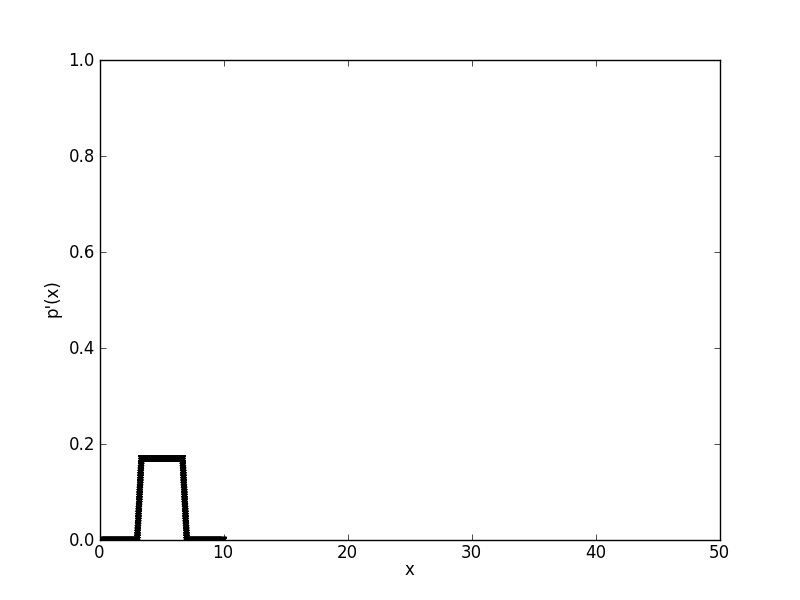
\includegraphics[width=0.4\textwidth]{graph1.png}
    }
    \subfigure[Regra 2]{
    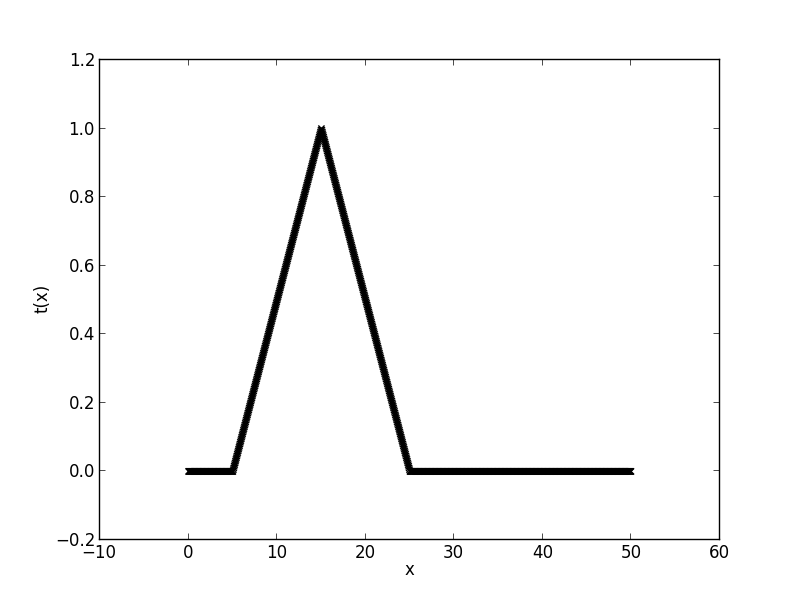
\includegraphics[width=0.4\textwidth]{graph2.png}
    }
    \end{center}
    \caption{Temperatura = $13,3^oC$}
\end{figure}


\begin{figure}[h!]
\begin{center}
    \subfigure[Regra 2]{%
    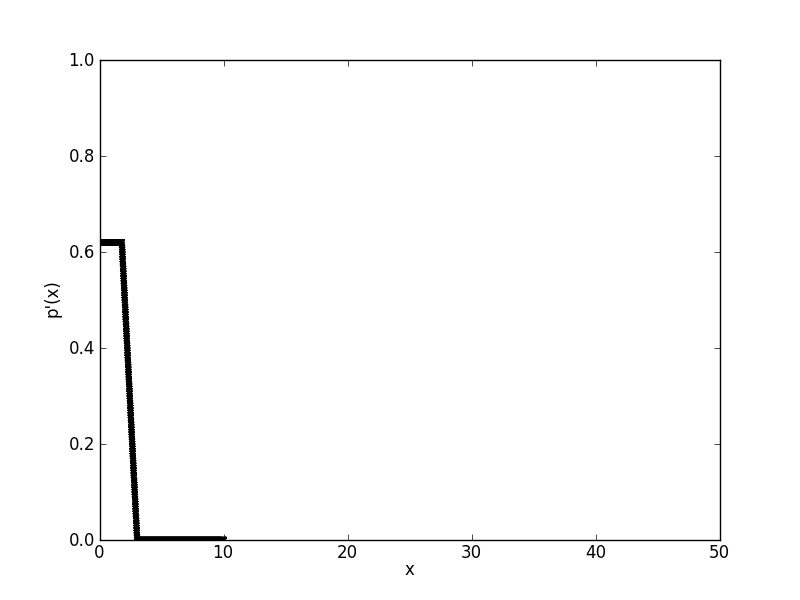
\includegraphics[width=0.4\textwidth]{graph3.png}
    }
    \subfigure[Regra 3]{
    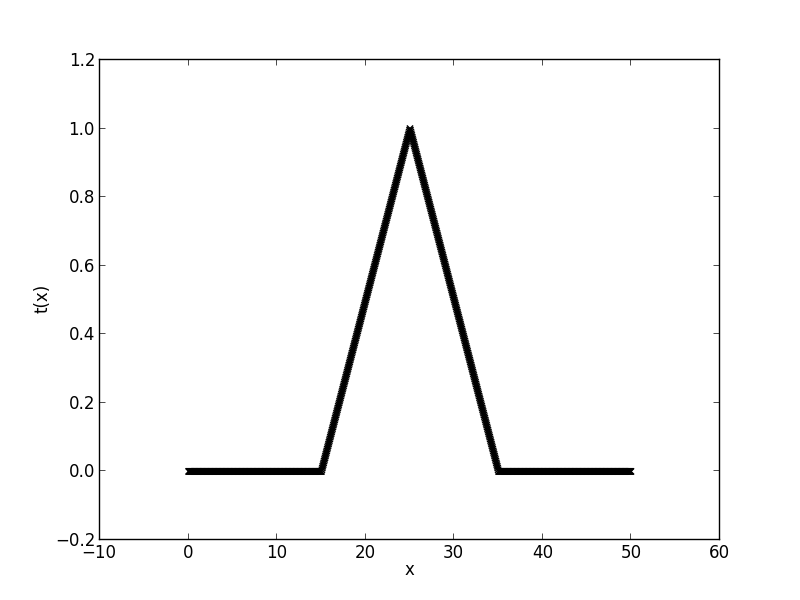
\includegraphics[width=0.4\textwidth]{graph4.png}
    }
    \end{center}
    \caption{Temperatura = $18,8^oC$}
\end{figure}

\begin{figure}[h!]
\begin{center}
    \subfigure[Regra 3]{%
    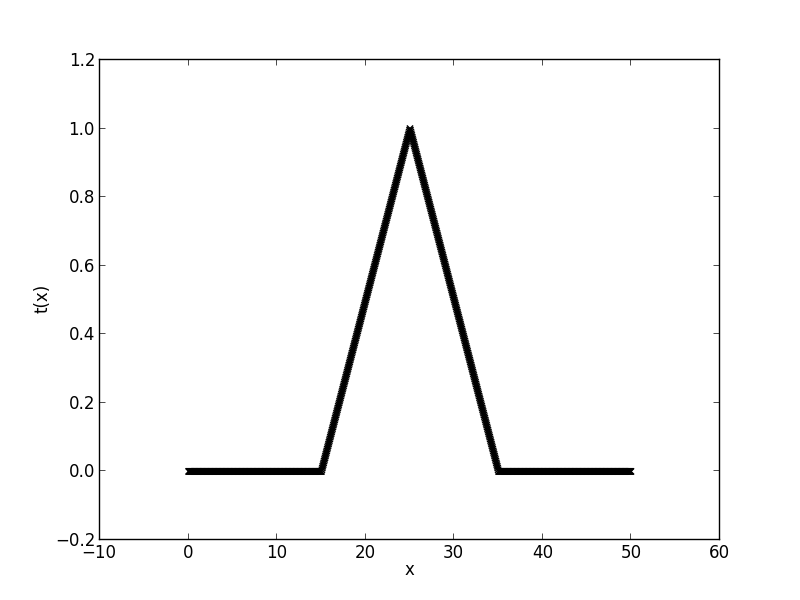
\includegraphics[width=0.4\textwidth]{graph5.png}
    }
    \subfigure[Regra 4]{
    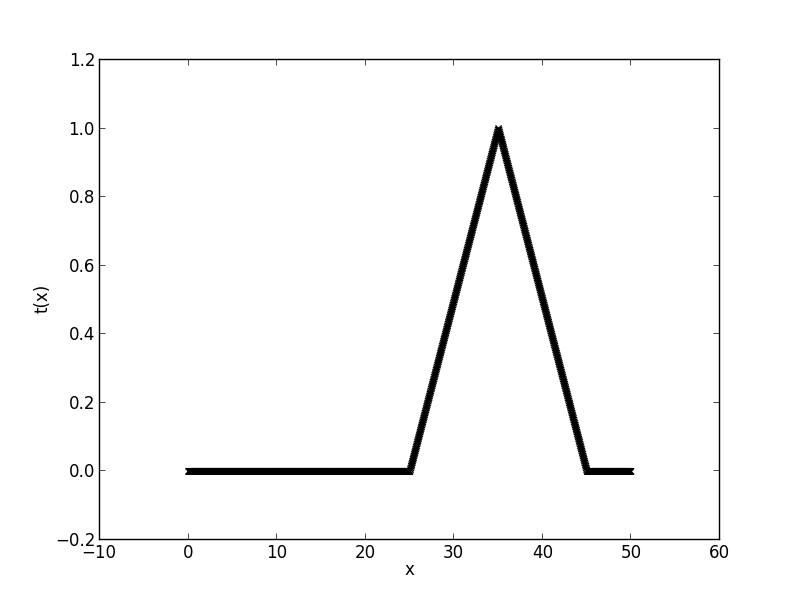
\includegraphics[width=0.4\textwidth]{graph6.png}
    }
    \end{center}
    \caption{Temperatura = $30,0^oC$}
\end{figure}

\begin{figure}[h!]
\begin{center}
    \subfigure[Regra 4]{%
    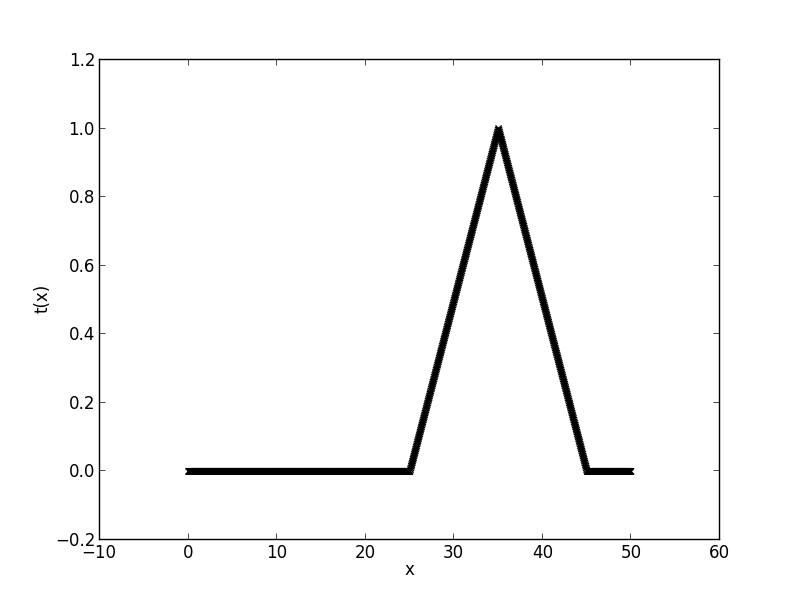
\includegraphics[width=0.4\textwidth]{graph7.png}
    }
    \subfigure[Regra 5]{
    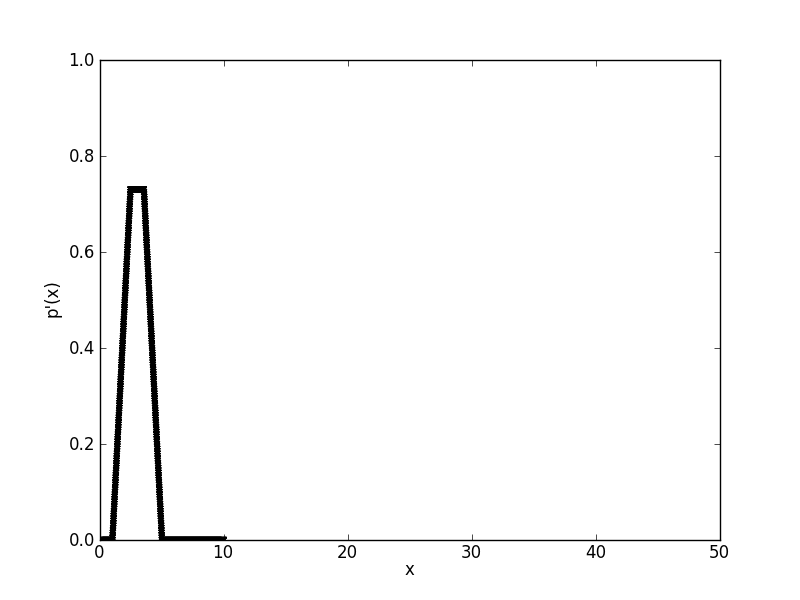
\includegraphics[width=0.4\textwidth]{graph8.png}
    }
    \end{center}
    \caption{Temperatura = $42,3^oC$}
\end{figure}

\begin{figure}[h!]
\begin{center}
    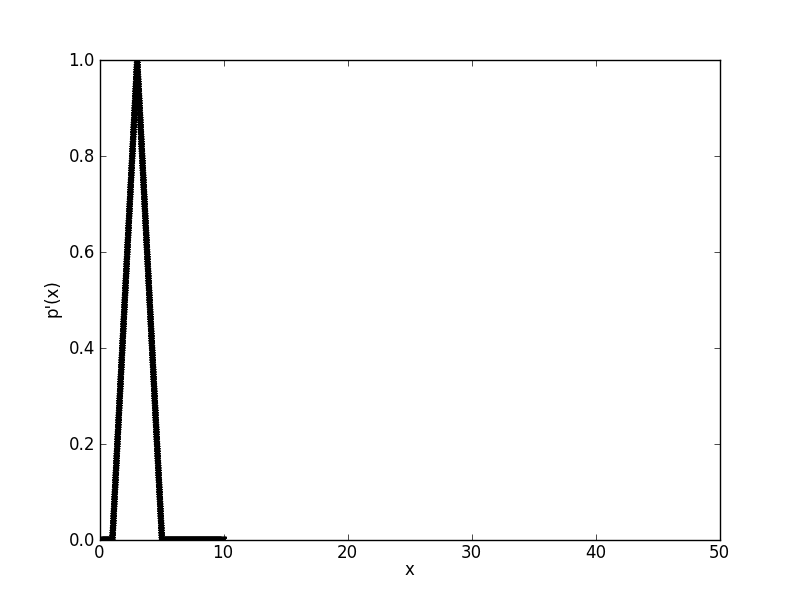
\includegraphics[width=0.4\textwidth]{graph9.png}
    \end{center}
\caption{Temperatura = $47,0^oC$}
\end{figure}

\newpage
\item[4.] A seguir encontram-se os gráficos de p'(x) utilizando o operador de Zadeh.

\begin{figure}[h!]
\begin{center}
    \subfigure[Regra 1]{%
    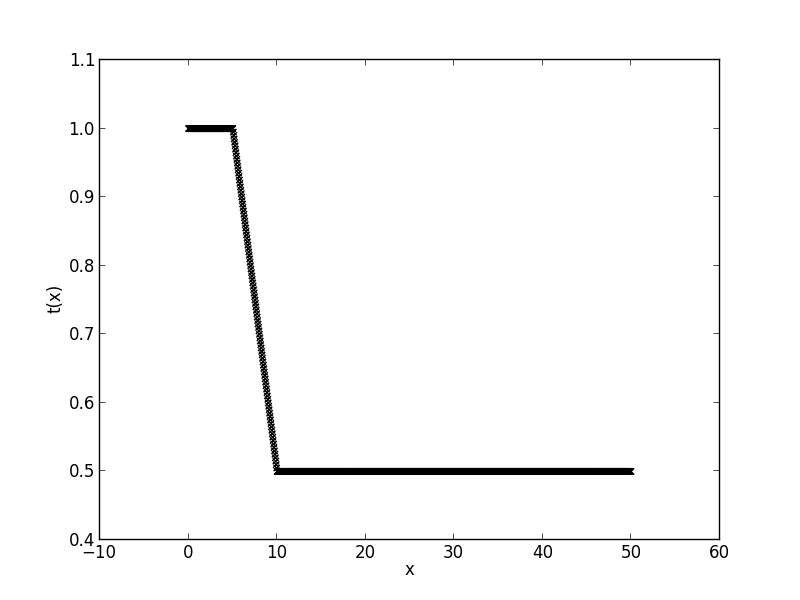
\includegraphics[width=0.4\textwidth]{graph10.png}
    }
    \subfigure[Regra 2]{
    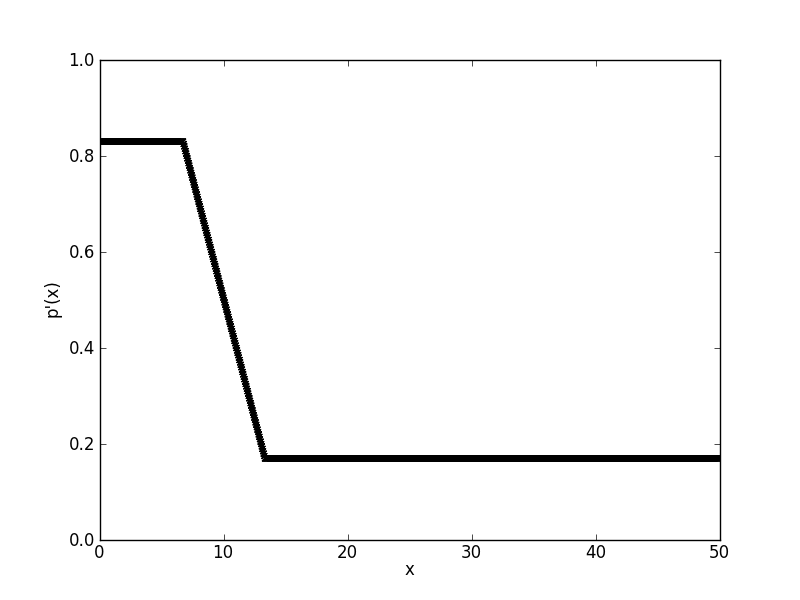
\includegraphics[width=0.4\textwidth]{graph11.png}
    }
    \end{center}
    \caption{Temperatura = $13,3^oC$}
\end{figure}


\begin{figure}[h!]
\begin{center}
    \subfigure[Regra 2]{%
    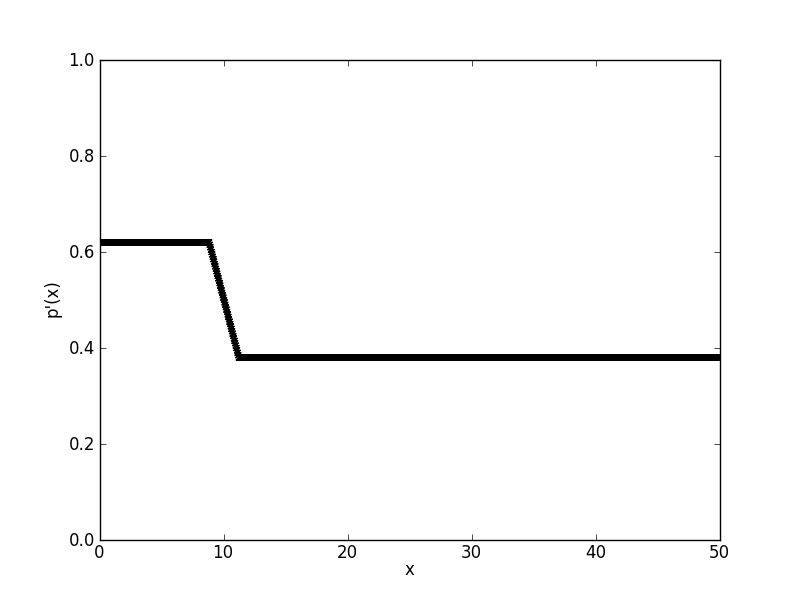
\includegraphics[width=0.4\textwidth]{graph12.png}
    }
    \subfigure[Regra 3]{
    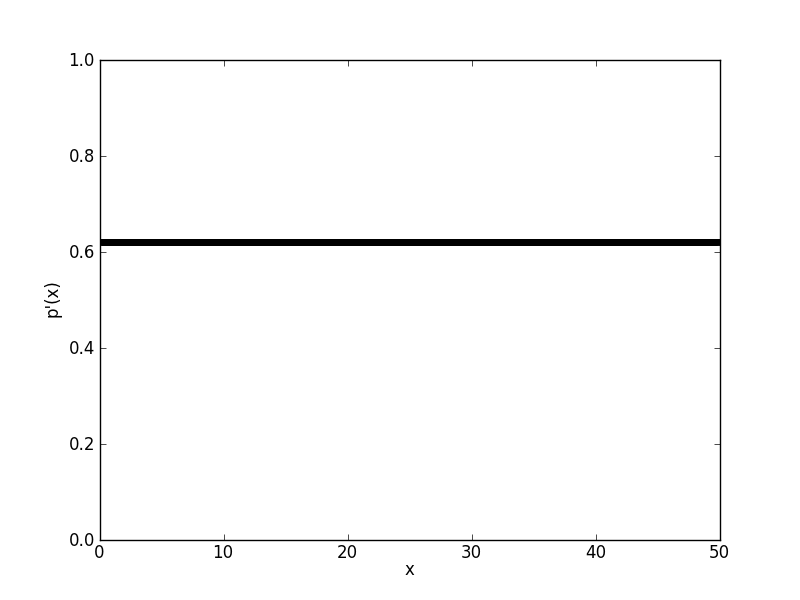
\includegraphics[width=0.4\textwidth]{graph13.png}
    }
    \end{center}
    \caption{Temperatura = $18,8^oC$}
\end{figure}

\begin{figure}[h!]
\begin{center}
    \subfigure[Regra 3]{%
    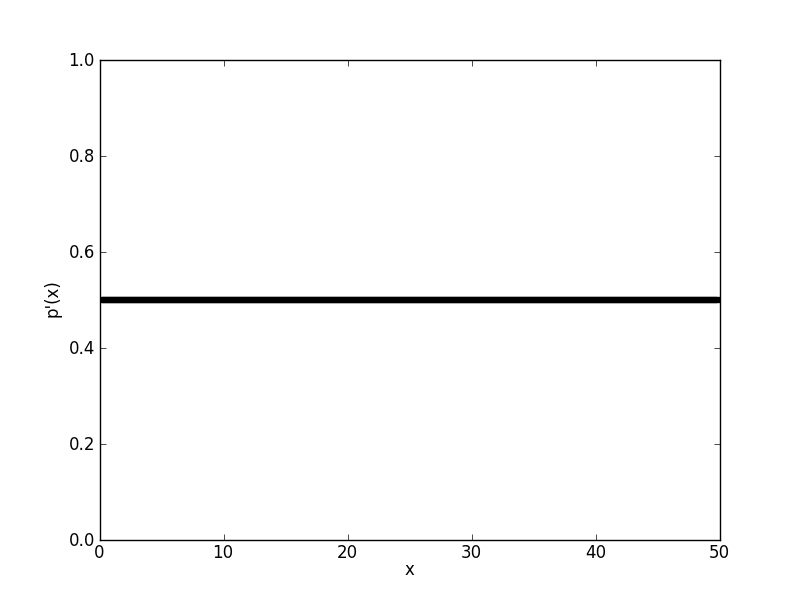
\includegraphics[width=0.4\textwidth]{graph14.png}
    }
    \subfigure[Regra 4]{
    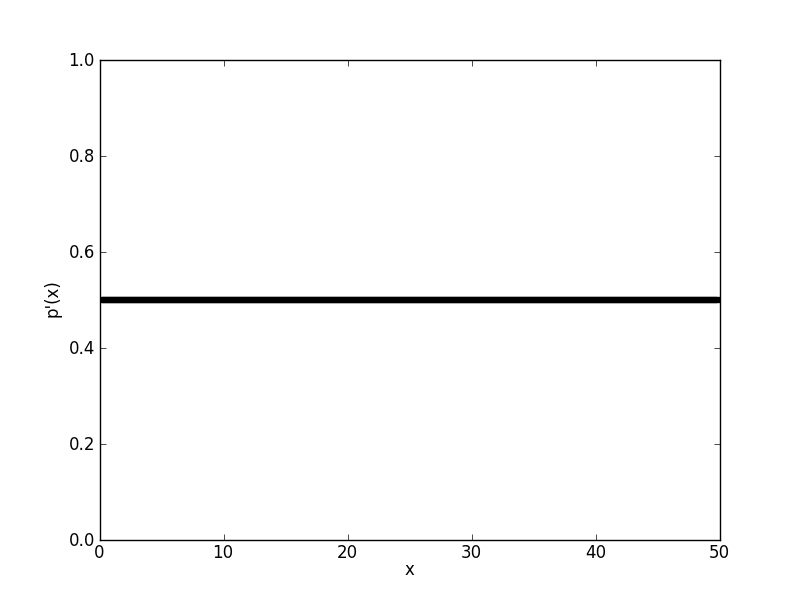
\includegraphics[width=0.4\textwidth]{graph15.png}
    }
    \end{center}
    \caption{Temperatura = $30,0^oC$}
\end{figure}

\begin{figure}[h!]
\begin{center}
    \subfigure[Regra 4]{%
    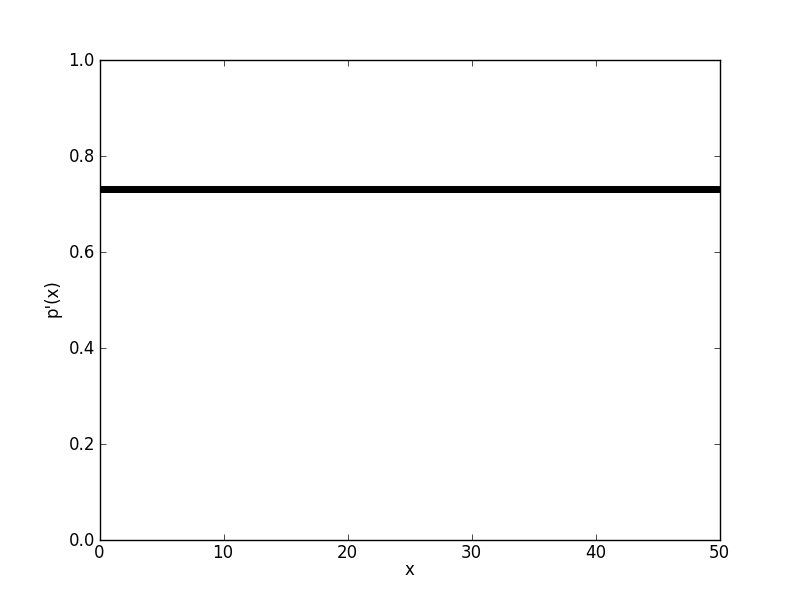
\includegraphics[width=0.4\textwidth]{graph16.png}
    }
    \subfigure[Regra 5]{
    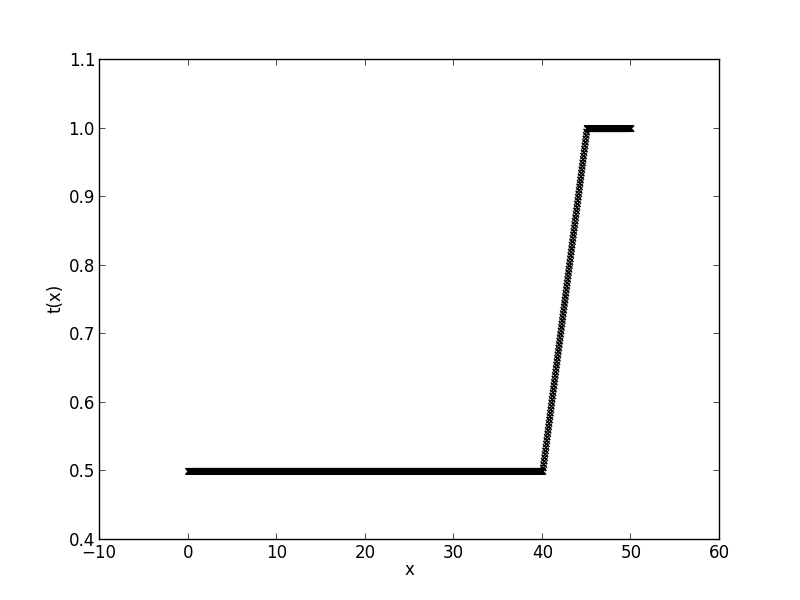
\includegraphics[width=0.4\textwidth]{graph17.png}
    }
    \end{center}
    \caption{Temperatura = $42,3^oC$}
\end{figure}

\begin{figure}[h!]
\begin{center}
    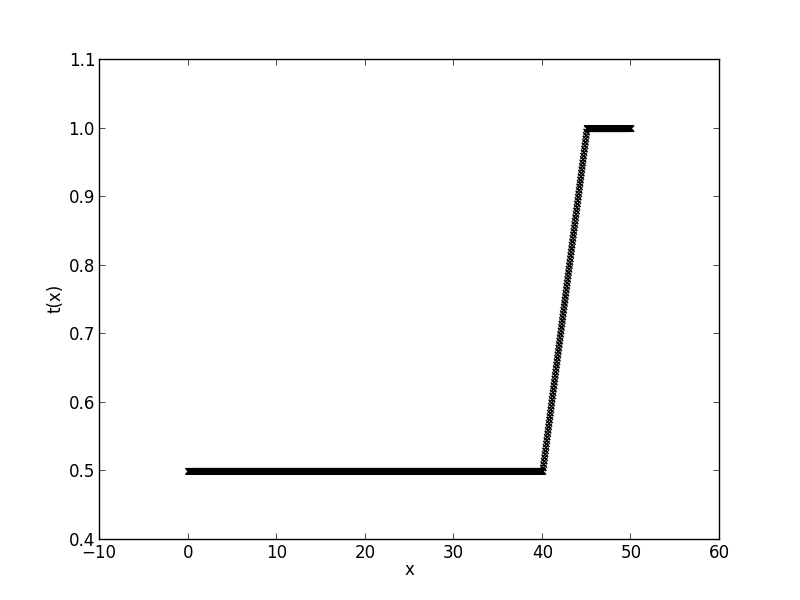
\includegraphics[width=0.4\textwidth]{graph18.png}
    \end{center}
\caption{Temperatura = $47,0^oC$}
\end{figure}


\cleardoublepage
\item[5.] A seguir encontram-se os gráficos de p'(x) utilizando o operador de Larsen.

\begin{figure}[h!]
\begin{center}
    \subfigure[Regra 1]{%
    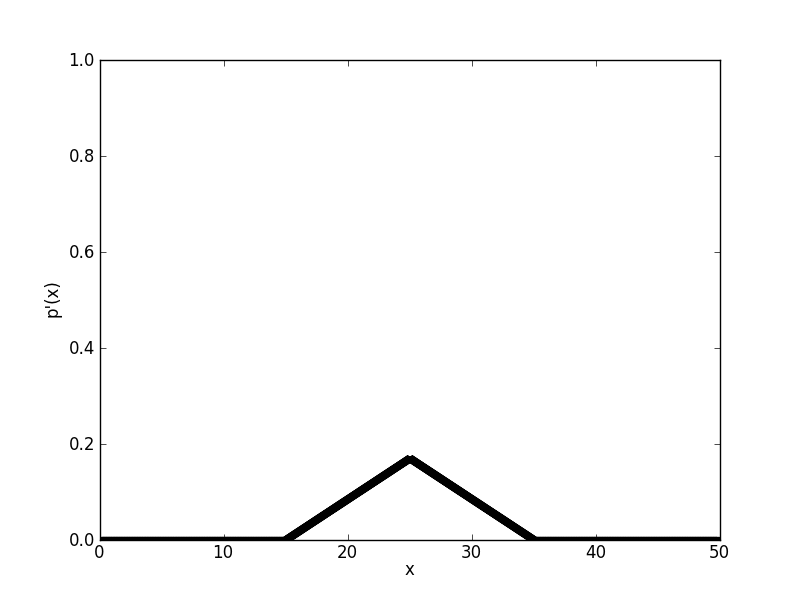
\includegraphics[width=0.4\textwidth]{graph19.png}
    }
    \subfigure[Regra 2]{
    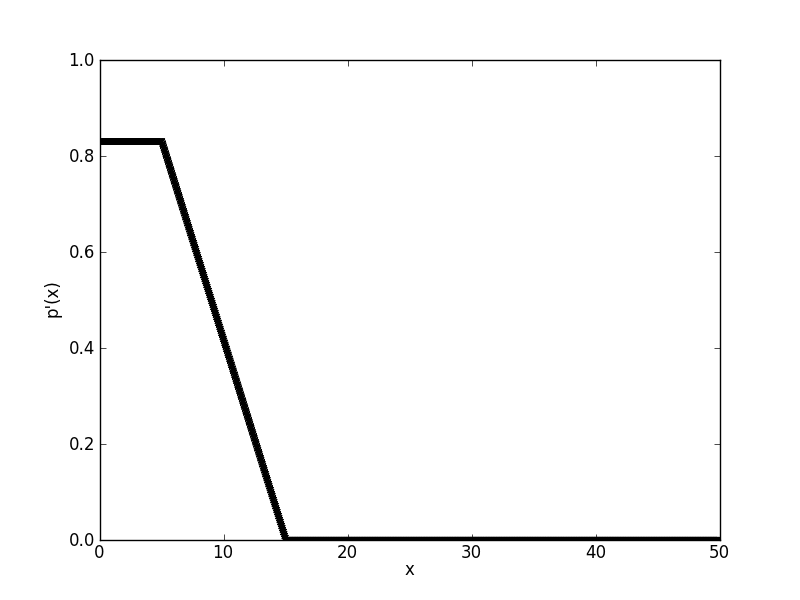
\includegraphics[width=0.4\textwidth]{graph20.png}
    }
    \end{center}
    \caption{Temperatura = $13,3^oC$}
\end{figure}


\begin{figure}[h!]
\begin{center}
    \subfigure[Regra 2]{%
    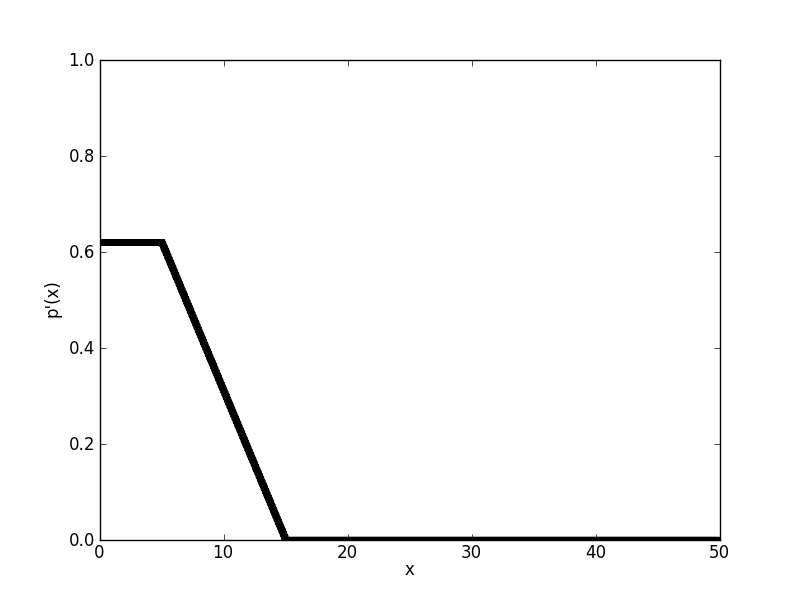
\includegraphics[width=0.4\textwidth]{graph21.png}
    }
    \subfigure[Regra 3]{
    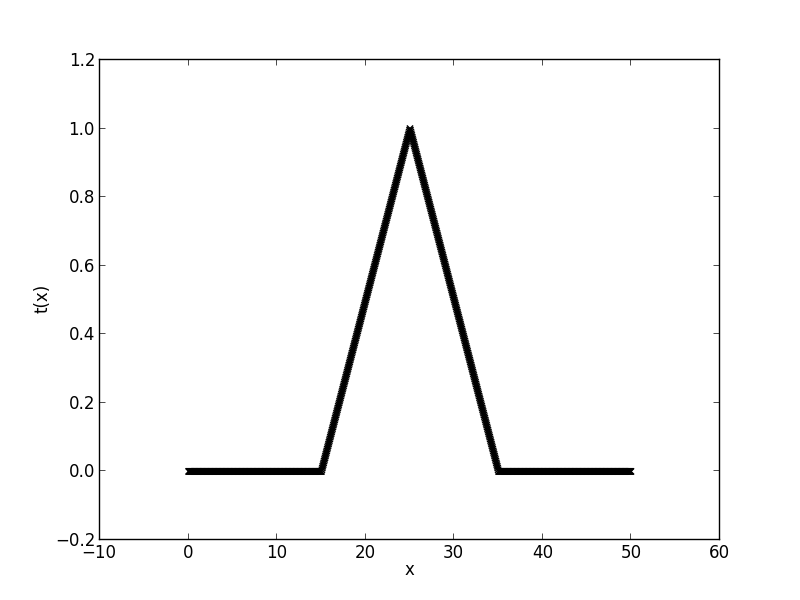
\includegraphics[width=0.4\textwidth]{graph22.png}
    }
    \end{center}
    \caption{Temperatura = $18,8^oC$}
\end{figure}

\begin{figure}[h!]
\begin{center}
    \subfigure[Regra 3]{%
    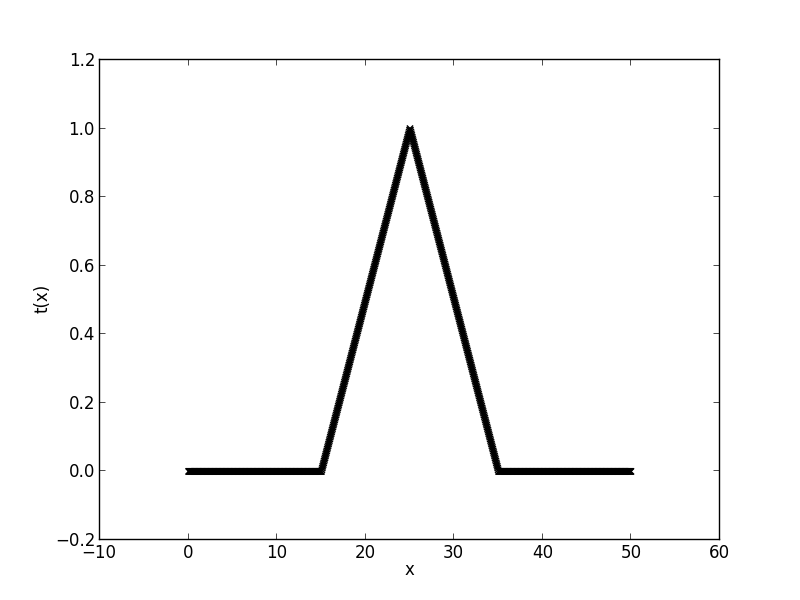
\includegraphics[width=0.4\textwidth]{graph23.png}
    }
    \subfigure[Regra 4]{
    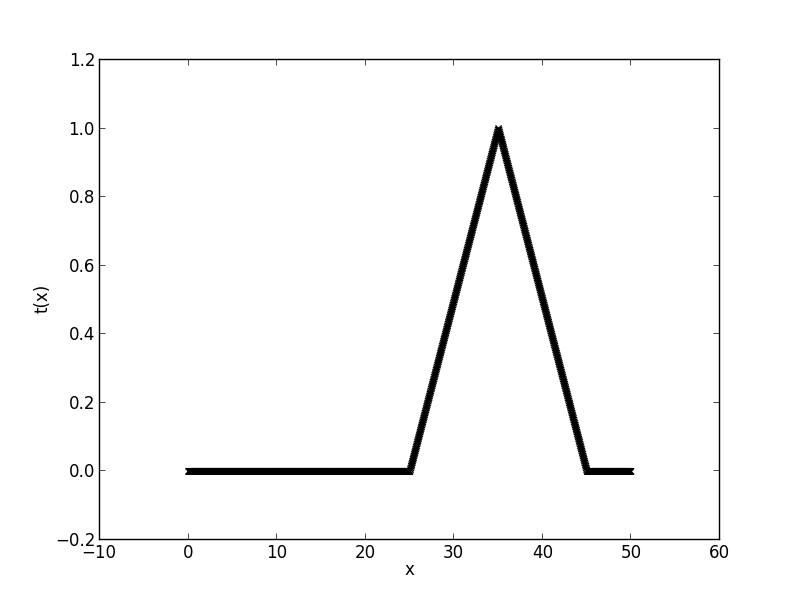
\includegraphics[width=0.4\textwidth]{graph24.png}
    }
    \end{center}
    \caption{Temperatura = $30,0^oC$}
\end{figure}

\begin{figure}[h!]
\begin{center}
    \subfigure[Regra 4]{%
    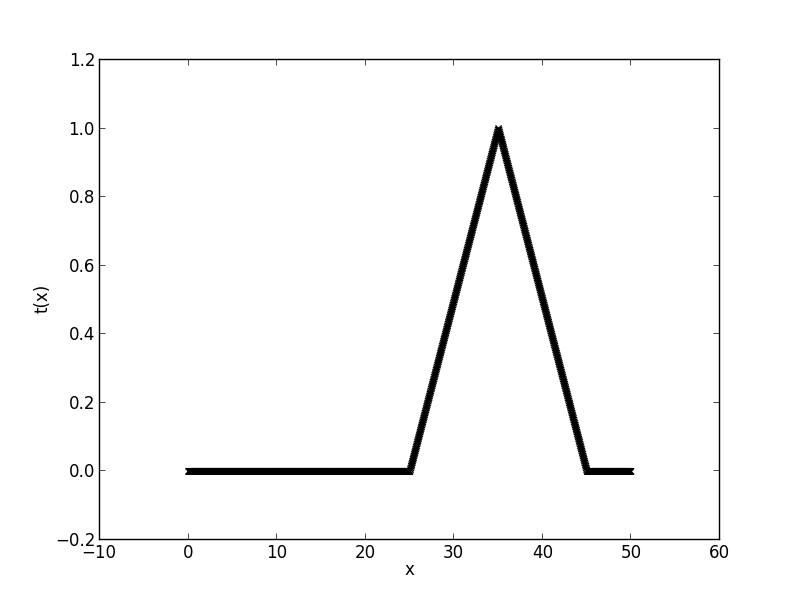
\includegraphics[width=0.4\textwidth]{graph25.png}
    }
    \subfigure[Regra 5]{
    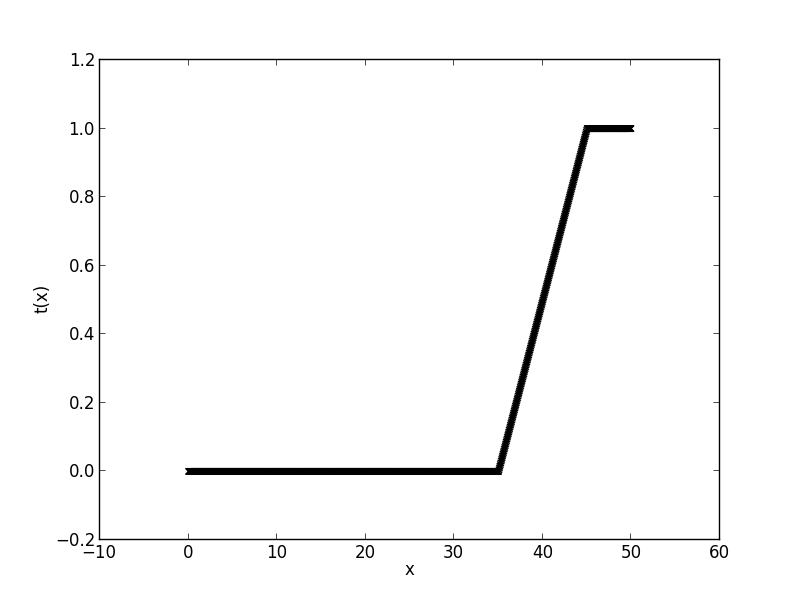
\includegraphics[width=0.4\textwidth]{graph26.png}
    }
    \end{center}
    \caption{Temperatura = $42,3^oC$}
\end{figure}

\begin{figure}[h!]
\begin{center}
    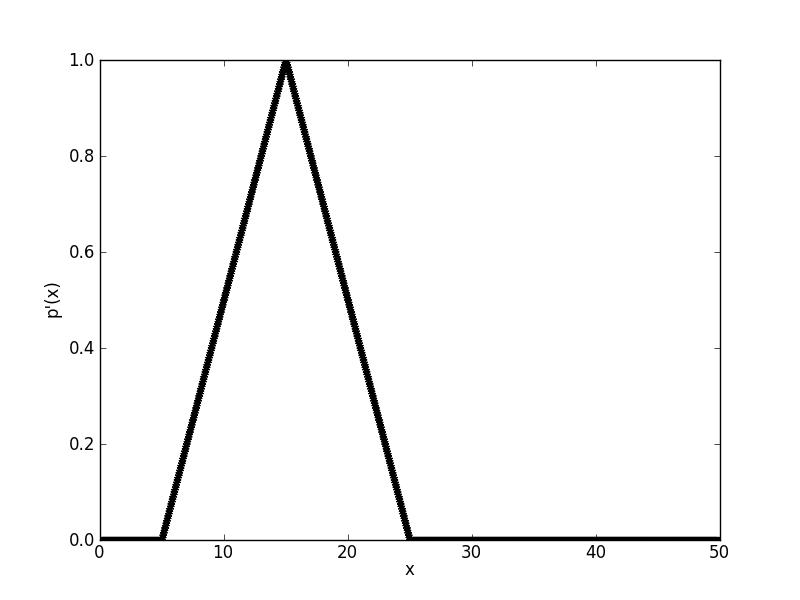
\includegraphics[width=0.4\textwidth]{graph27.png}
    \end{center}
\caption{Temperatura = $47,0^oC$}
\end{figure}



\end{enumerate}

\cleardoublepage
\lstinputlisting[language=Python]{epc5.py}
%\lstinputlisting{resp.txt}

\end{document}
